\RequirePackage{amsthm} %https://tex.stackexchange.com/questions/687324/unknown-theoremstyle-warning-with-springer-nature-template
\documentclass[sn-mathphys-num,iicol]{sn-jnl}

%\usepackage{sn-jnl.sty}
\usepackage{graphicx}%
\usepackage{multirow}%
\usepackage{amsmath,amssymb,amsfonts}%
\usepackage{amsthm}%
\usepackage{physics}
\usepackage{siunitx}
\usepackage{mathrsfs}%
\usepackage[title]{appendix}%
\usepackage{xcolor}%
\usepackage{textcomp}%
\usepackage{manyfoot}%
\usepackage{booktabs}%
\usepackage{algorithm}%
\usepackage{algorithmicx}%
\usepackage{algpseudocode}%
\usepackage{listings}%
\usepackage{newtxmath}%
\usepackage[tiny]{titlesec}%
\usepackage[ngerman]{babel}
\usepackage{booktabs}

\theoremstyle{thmstyleone}
\newtheorem{theorem}{Theorem}
\newtheorem{proposition}[theorem]{Proposition}

\theoremstyle{thmstyletwo}
\newtheorem{remark}{Remark}

\theoremstyle{thmstylethree}
\newtheorem{definition}{Definition}

\raggedbottom

\newcommand{\td}{\text{d}}

\titleformat{\subsection}{}{\thesubsection}{1em}{\itshape}
\titleformat{\subsubsection}{}{\thesubsubsection}{1em}{\itshape}

\begin{document}
        
\title[]{Praktikum 4 -- Versuch 422: Rastertunnelmikroskop}
\author*[1]{\fnm{Jonas} \sur{Wortmann}}\email{s02jwort@uni-bonn.de}
\author*[2]{\fnm{Angelo} \sur{Brade}}\email{s72abrad@uni-bonn.de}
\affil*[1,2]{Rheinische Friedrich--Wilhelms--Universität, Bonn}

\maketitle

\begin{figure}[h]
  \centering
  \begin{minipage}{.2\textwidth}
  \centering
  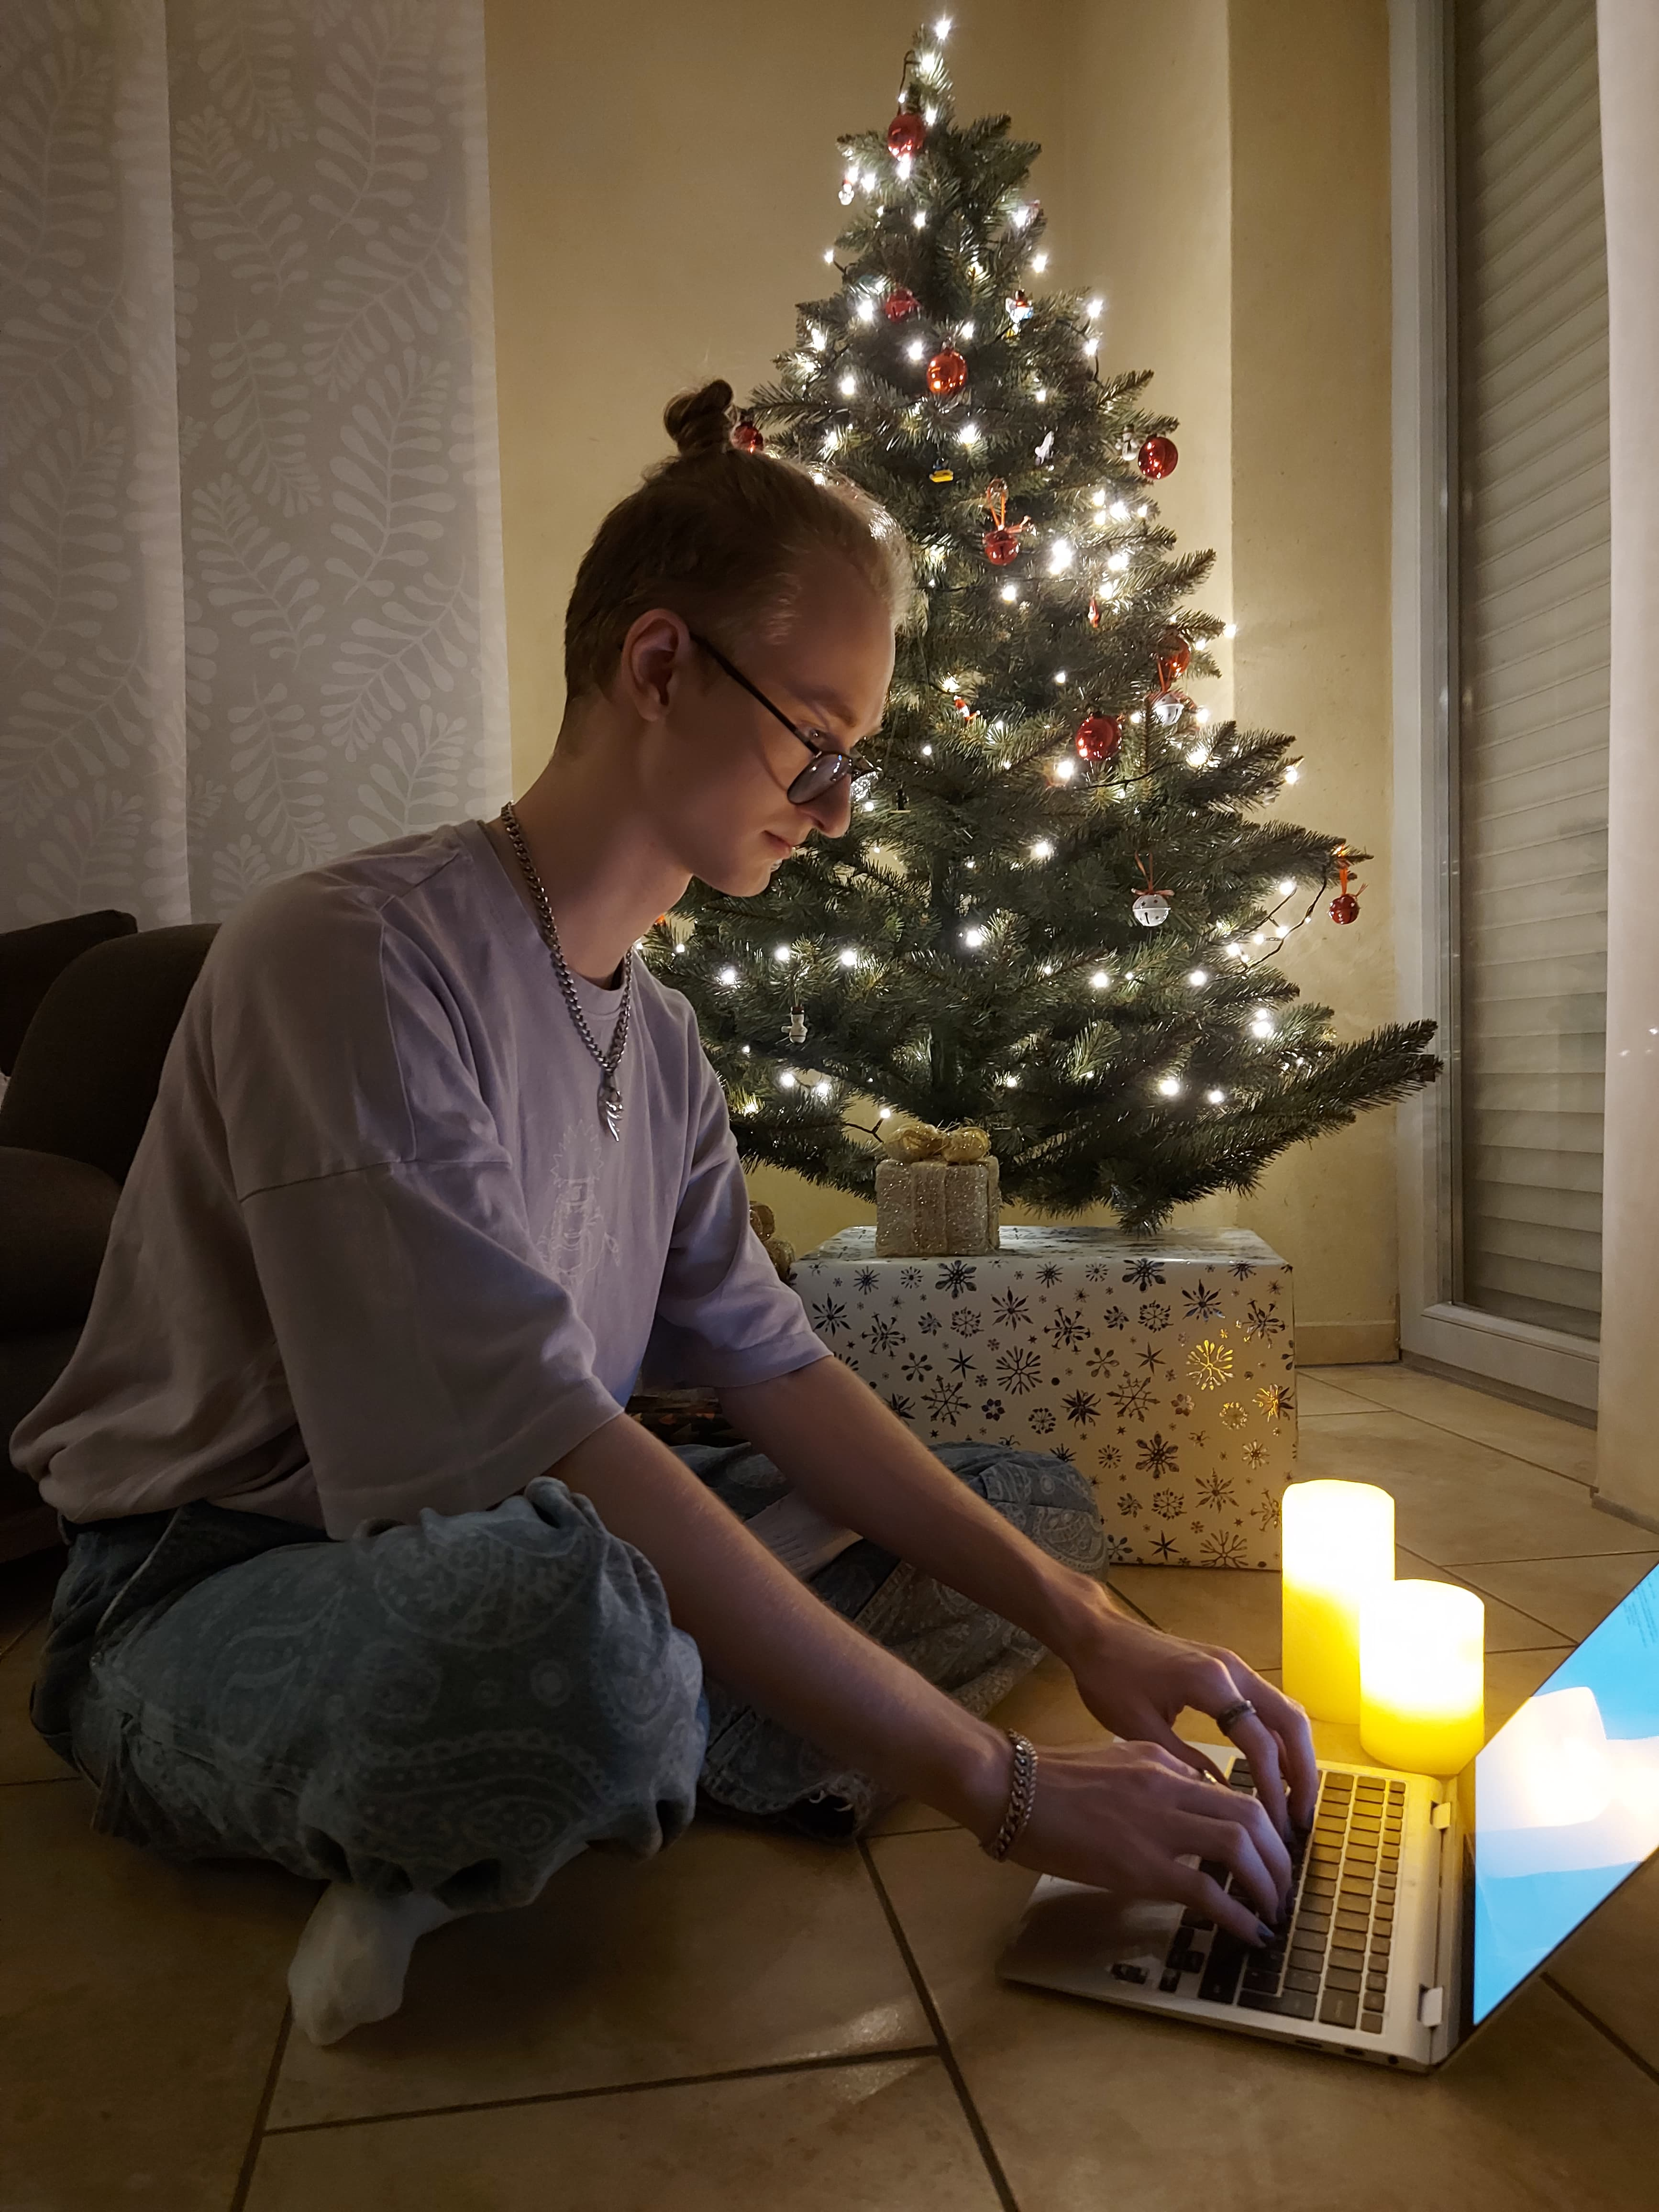
\includegraphics[width=\textwidth]{Jonas.jpeg}
  \end{minipage}
  \begin{minipage}{.2\textwidth}
  \centering
  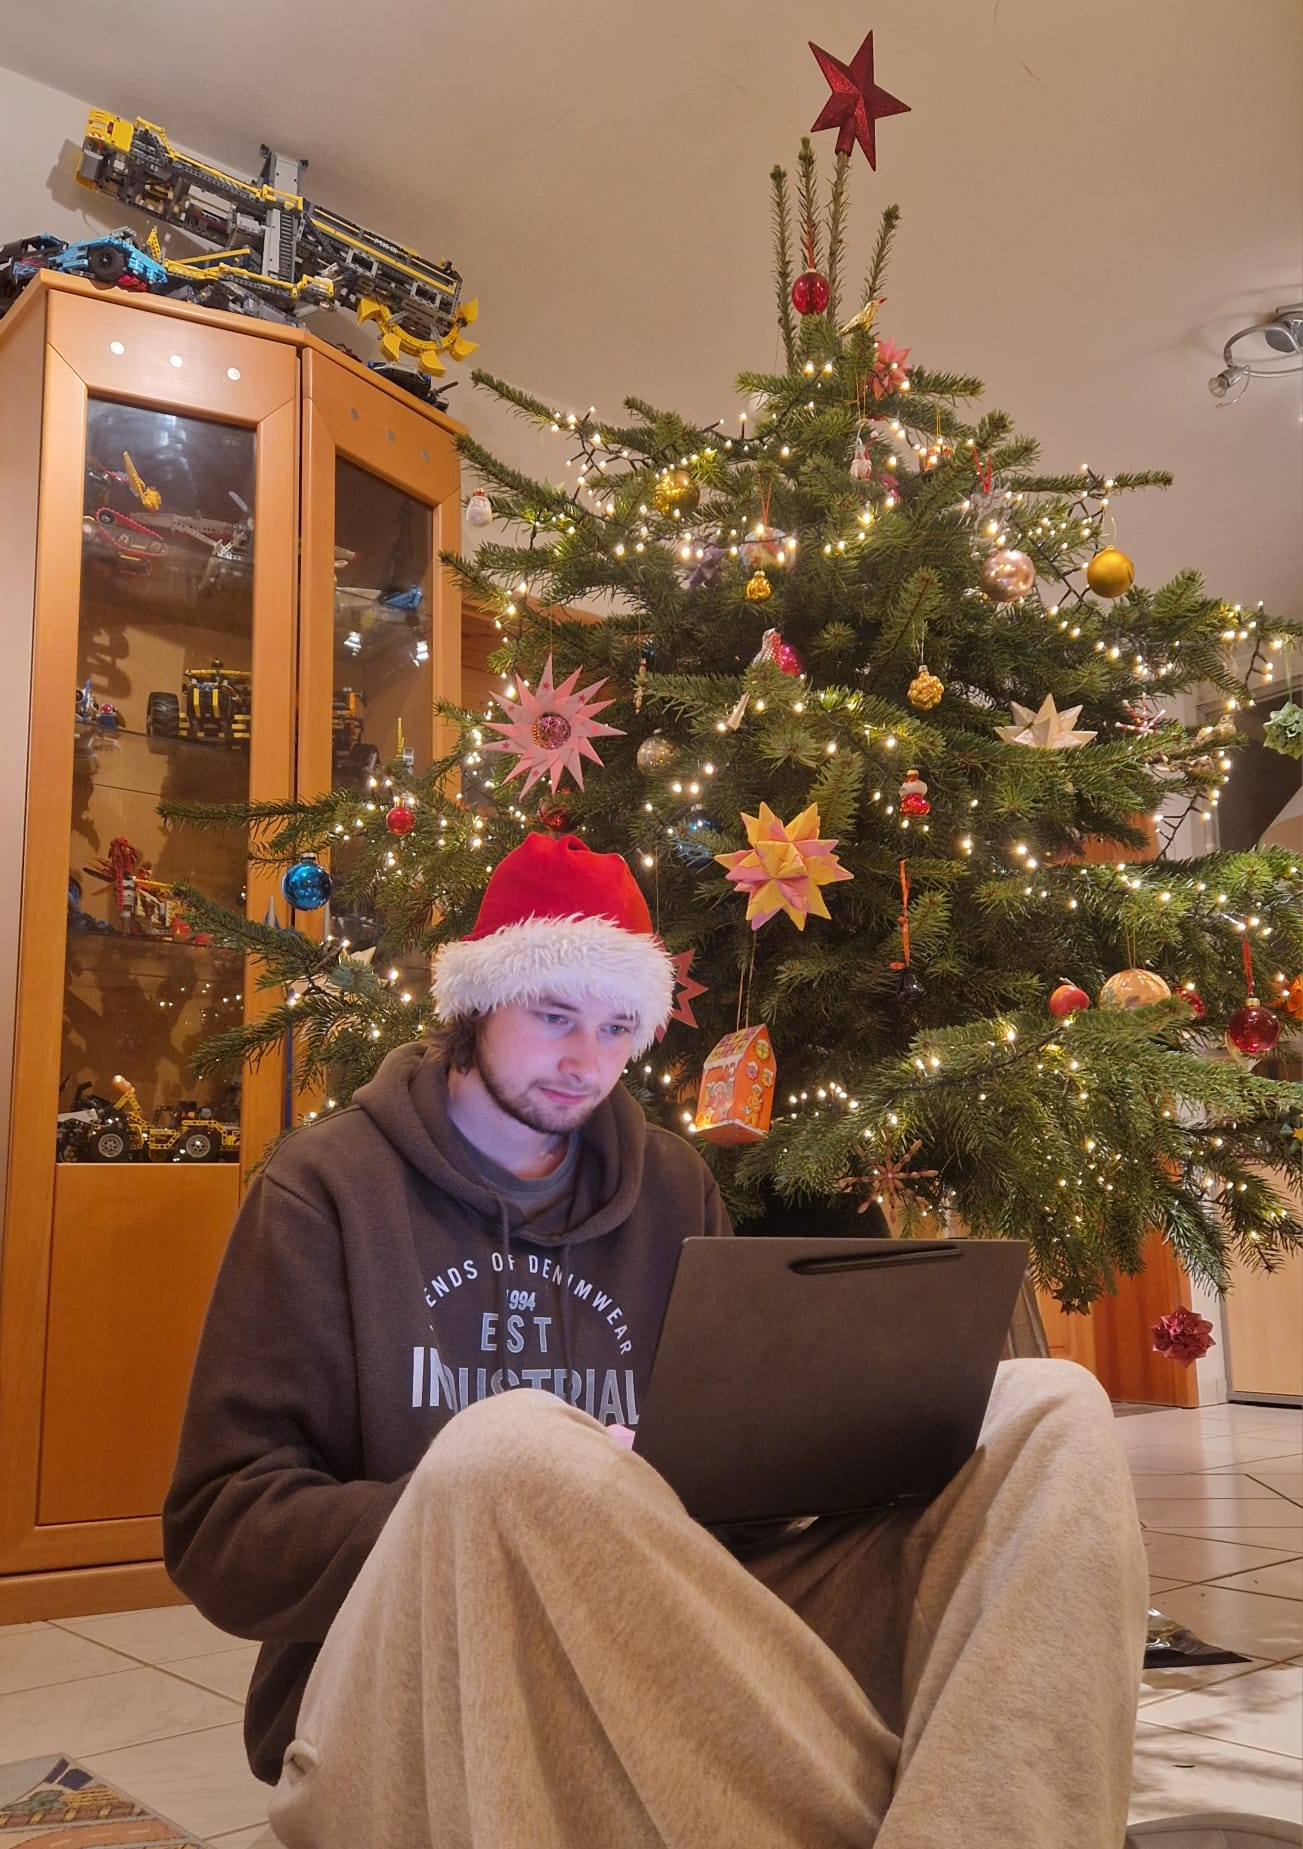
\includegraphics[width=.95\textwidth]{Angelo.jpeg}
  \end{minipage}
\end{figure}
%TODO sind die bilder hier so gut?

\section{Einleitung}
Um atomare Auflösungen und mikroskopische Materialstrukturen zu erkennen, ging aus der Vermessung von Austritsarbeiten eine neue Technologie hervor, die Vergrößerungen jenseits der optischen Begrenzung bietet.
Wenn sich zwei leitende Materialien mit verschiedenen Austrittsarbeiten nahe genug kommen, dann ist es Elektronen im \textsc{Fermi}--Niveau möglich, zwischen den Materialien zu tunneln.
Das Rastertunnelmikroskop (STM, scanning tunneling microscope) verwendet diesen Effekt, um Strukturen von Materialien auf mikroskopischer Ebene aufzulösen.

\section{Experimenteller Aufbau}
Der experimentelle Aufbau ist in Abb.\ (\ref{fig:aufbau}) zu sehen.
Das verwendete STM ist das \glqq NaioSTM\grqq{} von \textit{Nanosurf} (\url{www.nanosurf.com}).
\begin{figure}[t]
  \centering
  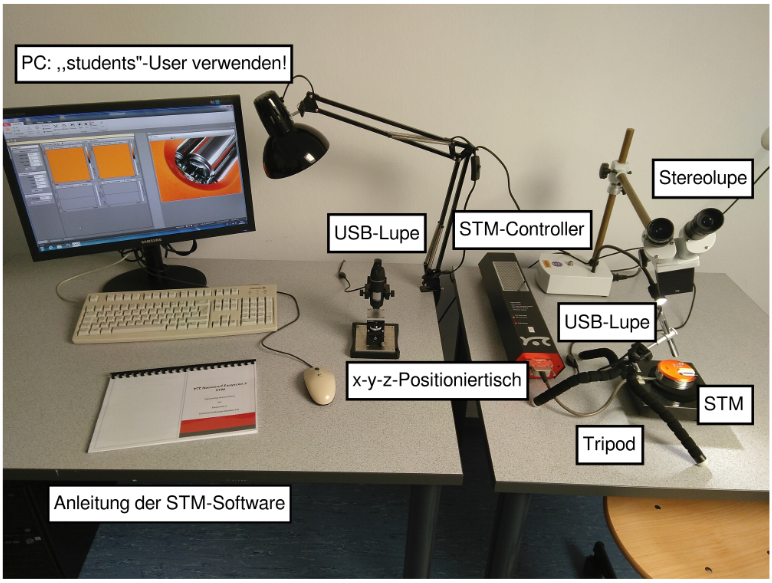
\includegraphics[width=.5\textwidth]{422_aufbau.png}
  \caption{Experimentiertisch.\cite{anleitung422}} \label{fig:aufbau}
\end{figure}
Das STM ist in Abb.\ (\ref{fig:naiostm}) zu sehen.
Der silberne Zylinder ist der Probenhalter, an dem die Probe mit einem Magneten festgehalten wird.
Der Probenhalter wird mit dem Slip--Stick Mechanismus bewegt.
Gegenüber der Probe ist eine Klammer, die einen Pt--Ir Draht hält (Abb.\ (\ref{fig:naiostm_closeup})).
Dieser ist die Spitze des Mikroskops.
Siehe auch Abb.\ (\ref{fig:spitze1}) und (\ref{fig:spitze2}).
\begin{figure}[t]
  \centering
  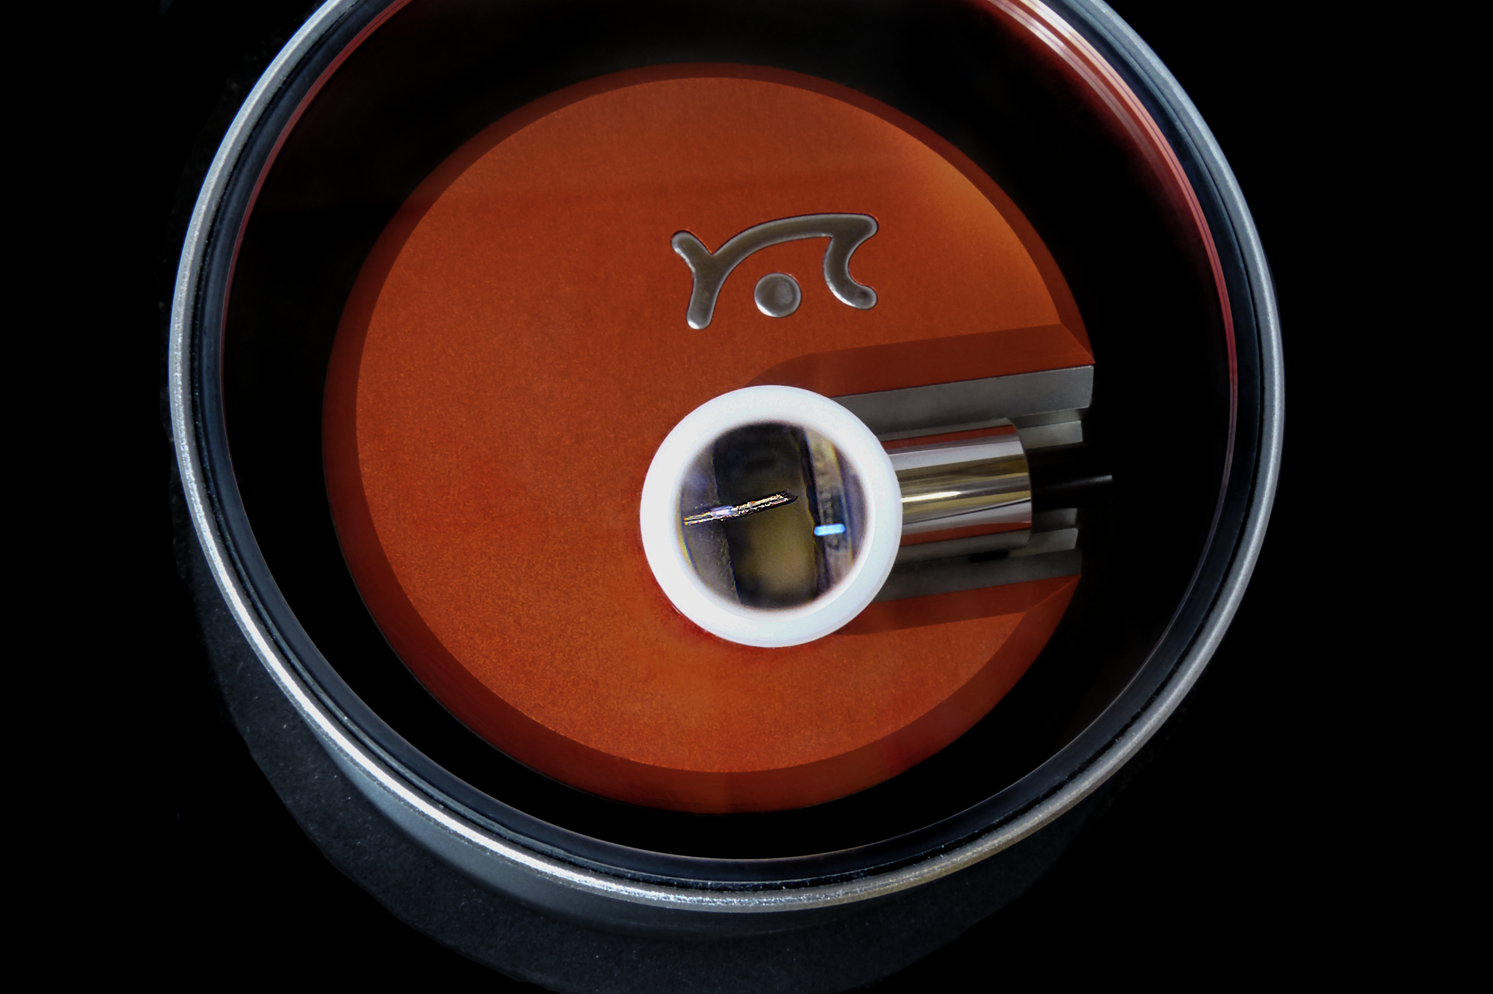
\includegraphics[width=.5\textwidth]{422_naiostm.png}
  \caption{NaioSTM von Nanosurf.\cite{nanosurf}} \label{fig:naiostm}
\end{figure}
\begin{figure}[t]
  \centering
  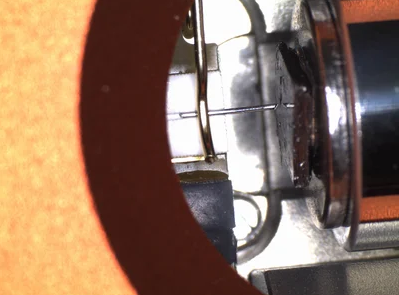
\includegraphics[width=.5\textwidth]{422_naiostm_closeup.png}
  \caption{NaioSTM von Nanosurf, Nahaufnahme der Spitze und Probe.\cite{nanosurf}} \label{fig:naiostm_closeup}
\end{figure}
\subsection{Theoretischer Hintergrund: STM}
Werden Spitze und Probe nah genug aneinander gefahren (s. Abb.\ (\ref{fig:naiostm_closeup})\footnote{Während der Messung sind Spitze und Probe in einem Abstand von wenigen zehntel Nanometer.}), so ist es den Elektronen im \textsc{Fermi}--Niveau der Probe möglich zur Spitze zu tunneln.
Dadurch entsteht ein Tunnelstrom.
Ein Bild der Probe wird erzeugt, in dem der gemessene Strom gegen den Ort aufgetragen wird.
Dieses Bild wird mit der \glqq Easyscan 2\grqq{} Software von Nanosurf aufgenommen.

Die Spitze kann mit makroskopischen Methoden von einem langen Pt--Ir Draht gewonnen werden.
Dabei wird ein kleines Stück des Drahtes mit einer Zange abgerissen, wodurch sich eine mikroskopisch kleine Spitze bildet. Das ist das sog. Reissen einer Spitze.
Da die Spitze nicht zu allen Seiten streng monoton fallend sein muss, sondern ausreichend ist, wenn es nur eine Stelle gibt, die der Probe am nächsten ist, kann diese Methode gut verwendet werden. % TODO: streng monoton fallend hört sich etwas over the top an // idk ich find das beschreibt es aber echt passend xD

Die Probe wird mit dem Slip--Stick Mechanismus an die Spitze herangefahren.
Dabei wird der Probenhalter mit einem anderen Material (z.B.\ Gummi) in Kontakt gebracht.
Da der Haftreibungskoeffizient größer als der Gleitreibungskoeffizient ist, kann durch langsame Bewegung des Gummis die Haftung zum Probenhalter erhalten bleiben und der Probenhalter wird verschoben.
Durch schnelles Zurückziehen des Gummis gleitet dies über den Probenhalter zurück in seine ursprüngliche Position und kann erneut am Probenhalter haften.

Die Bewegung der Probe orthogonal zur Spitze werden mit Hifle von \textsc{Piezo}--Kristallen realisiert.
Ein \textsc{Piezo}--Kristall besitzt in einer bestimmten Achse des Gitters keine Spiegelsymmetrie, wodurch mechanische Stauchung und Streckung eine Potentialdifferenz im Kristall verursachen.
Durch eine angelegte Spannung verschieben sich die Ladungsträger, wodurch eine Stauchung oder Streckung verursacht wird.
Dadurch wird die Probe (der Probenhalter) orthogonal zur Spitze verschoben.

Das STM kann in zwei Modi verwendet werden.

Im \textit{constant current mode} wird die Entfernung der Spitze von der Probe so reguliert, dass immer die gleiche Stromstärke gemessen wird.
Dies wird mit einem PID--Regelkreis (proportional integral differential) realisiert.
Die Einstellung hierfür sind $P=1000$, $I=2000$ und $D=0$.
Dieser Modus ist vor Allem für Proben mit unebenem Höhenprofil vorteilhaft, um die Spitze nicht auf der Probe auflaufen zu lassen.
Allerdings verringert sich in diesem Modus die Scangeschwindigkeit signifikant, da der Abstand der Spitze jedes mal neu justiert werden muss.

Im \textit{constant height mode} wird die Entfernung der Spitze von der Probe konstant gelassen.
Dies ermöglicht eine wesentlich schnellere Messung, ist allerdings nur für ebene Proben ratsam.
Die Einstellung des PID--Regelkreises sind $P=0$, $I=4$ und $D=0$.

\subsection{Maßstab}
Der Maßstab der Bilder des USB--Mikroskops wurde mit einem Gitter mit bekannten Maßstab gemessen.
Das Gitter in Abb.\ (\ref{fig:gitter_fern}) und (\ref{fig:gitter_nah}) besteht aus $\SI{400}{mm}\times \SI{100}{mm}$ Strichen.
Zu jedem mit dem USB--Mikroskop aufgenommenen Bild wurde der Maßstab anhand diesem Gitter abgelesen.

Der Maßstab der Bilder mit dem STM geht aus der Bildgröße hervor.

\section{Durchführung \& Auswertung:\\Goldprobe}
Die verwendete Goldprobe ist \glqq Gold14\grqq{} und in Abb.\ (\ref{fig:goldfern}), (\ref{fig:goldmittel}) und (\ref{fig:goldnah}) zu erkennen.
Die aufgenommenen Bilder sind (\ref{fig:g10nmc}), (\ref{fig:g10nmz}), (\ref{fig:g10nm50mVc}), (\ref{fig:g10nm50mVz}), (\ref{fig:g200nmc}), (\ref{fig:g200nmz}), (\ref{fig:g200nm50mVc}), (\ref{fig:g200nm50mVz}), (\ref{fig:g400nmc}) und (\ref{fig:g400nmz}).

In den makroskopischen Aufnahmen ist zu erkennen, dass die Goldprobe eine ebene Oberfläche besitzt, die durch viele Kratzer beschädigt ist.
Zudem sind drei prägnante Einkerbungen und ein runder Eindruck zu erkennen.
An diesen vier Stellen wurde die mikroskopische Untersuchung vermieden. % Das war uns egal lol, aber finde ich gut
Der Zusand dieser Probe ist für diesen Versuch föllig ausreichend. % Finde ich fr ein gutes Statement

\subsection{Untersuchung STM: \textit{constant current mode}}
Der \textit{constant current mode} wurde hier aufgrund der vielen Kratzer und Rauheit der Oberfläche verwendet, um die Spitze nicht zu beschädigen.

In Abb.\ (\ref{fig:g400nmc}) ist eine helle Wolke mit grauen Verschmierungen zu erkennen. 
Eine genauere Auflösung der Wolke ist in Abb.\ (\ref{fig:g200nmz}) und (\ref{fig:g200nm50mVz}), wobei die grauen Unterteilungen deutlich werden.
Dieser Bilder waren erwartet, da bei Gold das \textsc{Fermi}--Niveau im Leiterband ist und eine Auflösung des Gitters daher nicht möglich ist.
Abb.\ (\ref{fig:g10nmz}) und (\ref{fig:g10nm50mVz}) sind für die Auflösung der Wolken zu nah an der Probe.
Eine Aussage über die makroskopische Beschaffenheit der Oberfläche lässt sich hiermit nicht tätigen, allerdings kann erkannt werden, dass die Wolken ein Streifenmuster aufweisen.

Alle Stromkarten (\ref{fig:g10nmc}), (\ref{fig:g10nm50mVc}), (\ref{fig:g200nmc}), (\ref{fig:g200nm50mVc}) und (\ref{fig:g400nmc}) liefern identische Ergebnisse auf unterschiedlichen Größenskalen.
Es ist eine fast uniforme Stromverteilung zu erkennen mit vereinzelten sehr hellen Pixeln.
Dieses Ergebnis war erwartet, da hier im \textit{constant current mode} gearbeitet worden ist.

Es ist wichtig zu erwähnen, dass alle Abbildungen zu Gold Eigenschaften besitzen (z.B.\ Artefakte wie weiße Pixel und Striche) in dem Handbuch unter dem Kapitel zu nicht richtig aufgenommenen Bildern gelistet sind.
Es besteht also weiterhin die Möglichkeit, dass diese Bilder keine korrekten Aussagen über die Oberfläche geben.
Dies geht vor Allem aus dem Vergleich mit den Literaturaufnahmen in Abb.\ (\ref{fig:gold_lit}) hervor, in denen die Goldstruktur klar zu erkennen ist.

\section{Durchführung \& Auswertung:\\HOPG--Probe}
Die verwendete HOPG (highly oriented pyrolytic graphite) Probe ist \glqq HOPG8\grqq{} und in Abb.\ (\ref{fig:graphitfern}), (\ref{fig:graphitmittel}) und (\ref{fig:graphitnah}) zu erkennen.
Die aufgenommenen Bilder sind Abb.\ (\ref{fig:gr4nm50nVc}), (\ref{fig:gr4nm50nVz}), (\ref{fig:gr100nm100nVc}), (\ref{fig:gr100nm100nVz}), (\ref{fig:gr100nm200nVc}), (\ref{fig:gr100nm200nVz}), (\ref{fig:gr10nm200nVc}), (\ref{fig:gr10nm200nVz}), (\ref{fig:gr2nm50nVc}), (\ref{fig:gr2nm50nVz}), (\ref{fig:gr2nm50nVc2}), (\ref{fig:gr2nm50nVz2}), (\ref{fig:gr2nm50nVc3}) und (\ref{fig:gr2nm50nVz3}).

\subsection{Beobachtung}
In den makroskopischen Aufnahmen ist eine äußerst unebene Struktur zu erkennen, welche aus quaderförmigen kristallartigen Strukturen besteht. % TODO: Welche makrsoskopischen Aufnahmen genau? Ich kann da garkeite Struktur erkennen. // idk so ein bisschen kann man da ja größere klötze sehen. hab mal 'prägnant' und so rausgenommen xD
Aufgrund der natürlichen Unordnung und Unebenheit der Struktur sind keine Unreinheiten oder Beschädigungen zu erkennen.
Für die Untersuchung wurde eine möglichst flache Stelle auf der Probe verwendet.

\subsection{Untersuchung STM: constant current mode}
Der \textit{constant current mode} wurde hier aufgrund der makroskopischen Unebenheiten verwendet, um die Spitze nicht in die Probe zu bewegen.

Die Untersuchung der Probe -- vor Allem die Auflösung der Gittersturktur -- stellte sich als unerwartet schwierig dar, sodass diese nicht beobachtet werden konnte.
Alle Höhenkarten weisen Artefakte, Rauschen oder Schlieren auf; alle Stromkarten weisen vor Allem Rauschen und wenige Unebenheiten auf.

Um eine atomare Auflösung zu erzielen wurden folgende Vorgehensweisen versucht:
Eine neue Spitze wurde aus einer alten Spitze gerissen und mit großer Vorsicht in den Spitzenhalter eingebaut.
Dabei ist die Spitze nicht in Berührung mit anderen Gegenständen gekommen.
Die HOPG Probe wurde mehrfach abgezogen und der Probenhalter gereinigt.
Beim Anbringen der Probe wurde darauf geachtet, dass eine möglichst ebene Fläche der Probe zur Spitze zeigt.
Das Heranfahren an die Probe wurde nur auf eine noch makroskopisch unterschiedbare Entfernung mit der Hand getan, die weitere Bewegung wurde mit \textit{Approach} und \textit{Advance} vollführt, sodass es nicht möglich war, dass Probe und Spitze in Berührung gekommen sind.
Ein \textit{Adjust Slope} wurde durchgeführt und ein \textit{Tip Cleaning Pulse} gegeben.
Die Bilder wurden ohne Erfolg mit verschiedenen PID Parametern, verschiedenen Geschwindigkeiten und verschiedenen Größenordnungen gemacht.
Auch das Klopfen auf den Tisch hat nicht funktioniert.
Alle Schritte wurden für mehrere Spitzen ($<5$) durchgeführt und jedes mal sorgfältig gearbeitet.
Es konnte kein Bild in atmoarer Auflösung erzielt werden; auch für sehr kleine Bildgrößen, bei denen ein Gitter eigentlich aufgelöst werden sollte (s.\ z.B.\ Abb.\ (\ref{fig:gr10nm200nVz}))

In den Literaturbildern aus Abb.\ (\ref{fig:hopg_lit}) erkennt man die Gitterstruktur klar.
Vergleicht man mit den aufgenommenen Bildern sind die Unterschiede eindeutig.

\subsection{Gitterstruktur}
Da die Bilder keine verwertbare Gitterstruktur zeigen, kann hier die Bestimmung der Winkel und der Abstände zwischen den Atomen nicht berechnet werden.
Eine theoretische Berechnung sähe wie folgt aus:

Man wählt einen Bereich der Aufnahme, in der wenig Verzerrungen vorhanden sind, um möglichst einheitliche Abstände und Winkel zu betrachten.
Der Winkel zweier Atome kann über Vektoren berechnet werden.
Es gilt
\begin{align} 
  \alpha =\arccos\left(\dfrac{\boldsymbol{i} \boldsymbol{j} }{ij}\right)
,\end{align} 
mit $\boldsymbol{i} \equiv\vv{i}$ und $i\equiv |\vv{i}|$.
Die Vektoren ergeben sich aus der Verbindungslinie zweier Atome $A$ und $B$ oder $B$ und $C$
\begin{align} 
  \boldsymbol{i} =\overline{AB}=\text{Pos}(B)-\text{Pos}(A)\\
  \boldsymbol{j} =\overline{BC}=\text{Pos}(B)-\text{Pos}(C)
\end{align} 
wobei $A$ und $B$ die Koordinaten beider Atome von einem einheitlichen Ursprung gemessen sind.

Der Abstand zweier Atome kann mit Hilfe des Winkels berechnet werden.
Es ist für ein Hexagon
\begin{align} 
  \cos \ang{30}=\dfrac{1}{2}\dfrac{j}{i}\Leftrightarrow i=\dfrac{j}{2\cos \ang{30}}
,\end{align} 
mit $\ang{30}\equiv \tfrac{\alpha }{4}$.
%TODO meinst du hier muss noch mehr hin? der abschnitt ist recht kurz glaub ich aber tbh haben wir auch keine daten

% TODO: Vielleicht sollte auch nochmal diskutiert werden, dass wir nur eine einzige constant hight Aufnahmen haben. Außerden könnte die auch nochmal inhaltlich diksutiert werden. // wo is die denn?
\section{Fazit}
In diesem Versuch wurden Gold-- und HOGP--Proben untersucht, indem Bilder mit Hilfe eines STMs aufgenommen worden sind.
Die Verwendung des STM hat gut funktioniert, darunter auch das Spitzen reißen und einsetzen, sowie das Annähern der Probe an die Spitze.

Diese Bilder liefern für Gold gute Ergebnisse und zeigen eine wolkenartige Struktur, die für dieses Material erwartet war.
Dies ist auf unterschiedlichen Größenskalen zu erkennen.

Die Bilder der HOPG Probe zeigen keine brauchbaren Ergebnisse.
Hier ist die erwartete Gitterstruktur auf verschiedenen Größenskalen nicht zu erkennen.
Mögliche Ursachen hierfür könnten unter anderem eine fehlerhafte Spitze oder falsche Bedienung des STMs sein.
Die angestellten Methoden zur Verbesserung der Bildqualität haben nicht funktioniert.
Die Berechnung der Winkel und Abstand zwischen den Atomen hat mit diesen Aufnahmen auch nicht funktioniert.

\bibliography{refs}

\clearpage
\section{Appendix}
\begin{figure}[h]
  \centering
  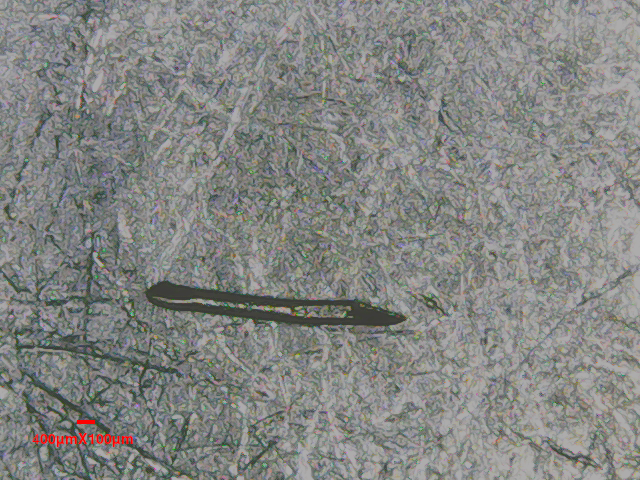
\includegraphics[width=.5\textwidth]{../data/Spitze1_1.png}
  \caption{Spitze 1.} \label{fig:spitze1}
\end{figure}
\begin{figure}[h]
  \centering
  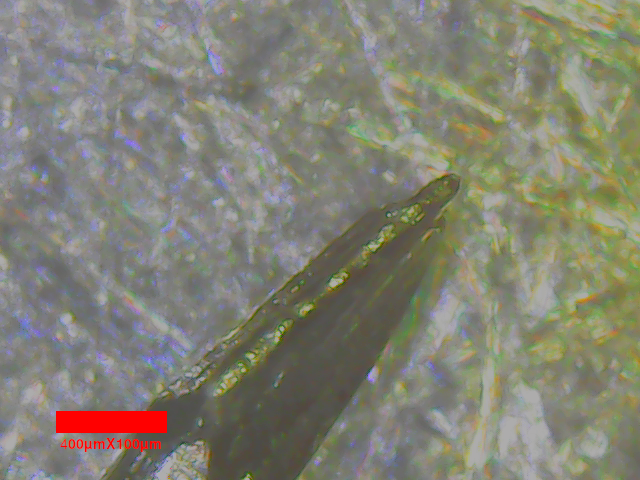
\includegraphics[width=.5\textwidth]{../data/Spitze1_2.png}
  \caption{Spitze 2.} \label{fig:spitze2}
\end{figure}
\clearpage
\begin{figure}[t]
  \centering
  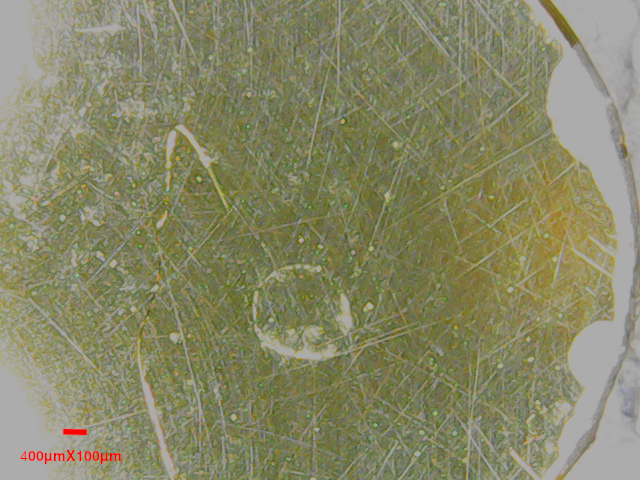
\includegraphics[width=.5\textwidth]{../data/Gold_1.png}
  \caption{Gold fern.} \label{fig:goldfern}
\end{figure}
\begin{figure}[t]
  \centering
  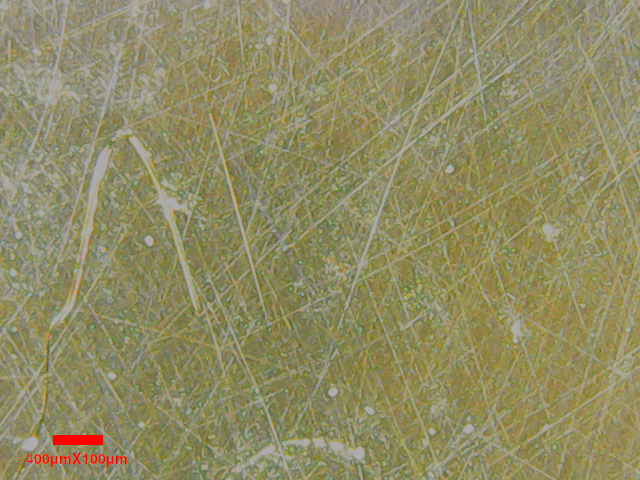
\includegraphics[width=.5\textwidth]{../data/Gold_2.png}
  \caption{Gold mittel.} \label{fig:goldmittel}
\end{figure}
\begin{figure}[t]
  \centering
  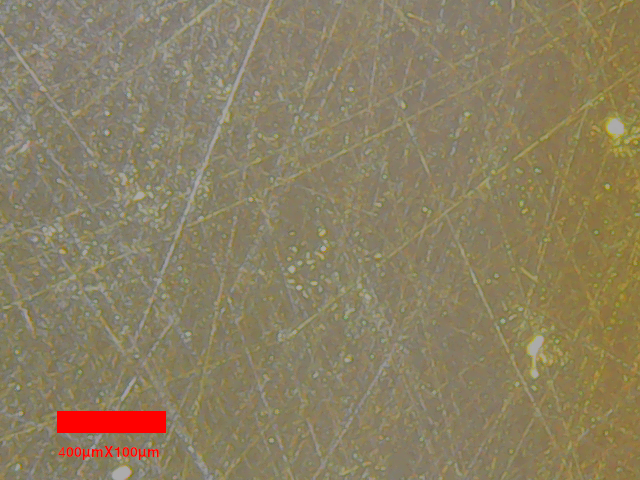
\includegraphics[width=.5\textwidth]{../data/Gold_3.png}
  \caption{Gold nah.} \label{fig:goldnah}
\end{figure}
\begin{figure}[t]
  \centering
  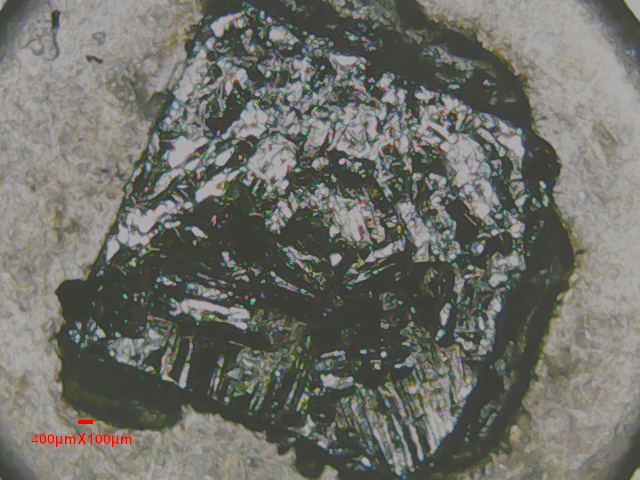
\includegraphics[width=.5\textwidth]{../data/Graphit_3.png}
  \caption{Graphit fern.} \label{fig:graphitfern}
\end{figure}
\begin{figure}[t]
  \centering
  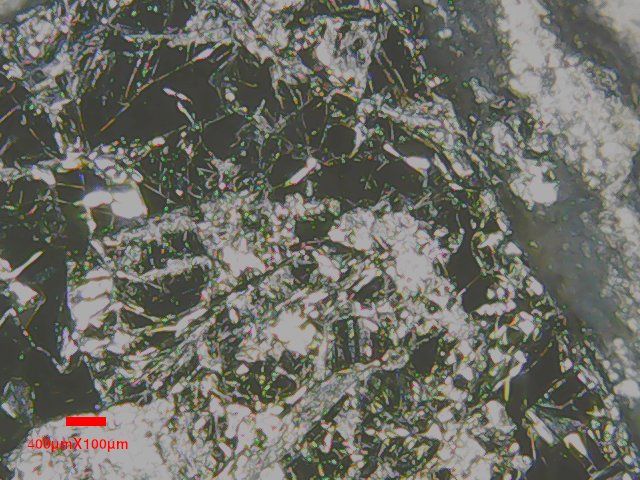
\includegraphics[width=.5\textwidth]{../data/Graphit_1.png}
  \caption{Graphit mittel.} \label{fig:graphitmittel}
\end{figure}
\begin{figure}[t]
  \centering
  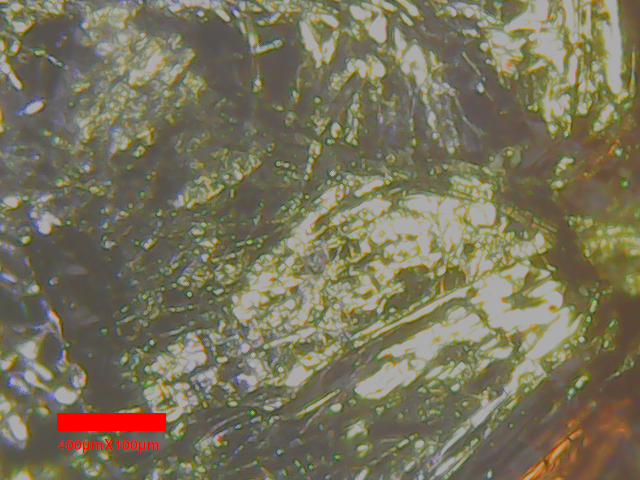
\includegraphics[width=.5\textwidth]{../data/Graphit_2.png}
  \caption{Graphit nah.} \label{fig:graphitnah}
\end{figure}
\clearpage

% TODO: Grobe aufteilung. Kann immer geändert werden. Ist jetzt nicht so festgelegt. Nur als Orientierung.
\section{Goldprobe}
\begin{figure}[h]
        \centering
        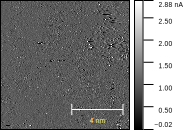
\includegraphics[width=.5\textwidth]{../data/Gold_10nm_current.png}
        \caption{Gold: Stromkarte im const. current Modus (Setpoint=\SI{1}{\nano A}, P-Gain=\SI{1000}{}, I-Gain=\SI{2000}{} und Tip voltage=\SI{1}{V})} \label{fig:g10nmc}
\end{figure}
\begin{figure}[h]
        \centering
        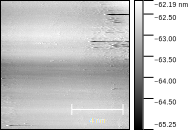
\includegraphics[width=.5\textwidth]{../data/Gold_10nm_z.png}
        \caption{Gold: Höhenkarte im const. current Modus (Setpoint=\SI{1}{\nano A}, P-Gain=\SI{1000}{}, I-Gain=\SI{2000}{} und Tip voltage=\SI{1}{V})} \label{fig:g10nmz}
\end{figure}
\begin{figure}[h]
        \centering
        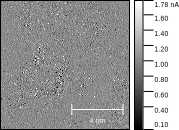
\includegraphics[width=.5\textwidth]{../data/Gold_10nm_50mV_current.png}
        \caption{Gold: Stromkarte im const. current Modus (Setpoint=\SI{1}{\nano A}, P-Gain=\SI{1000}{}, I-Gain=\SI{2000}{} und Tip voltage=\SI{50}{\milli V})} \label{fig:g10nm50mVc}
\end{figure}
\begin{figure}[h]
        \centering
        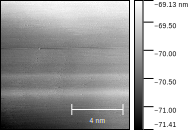
\includegraphics[width=.5\textwidth]{../data/Gold_10nm_50mV_z.png}
        \caption{Gold: Höhenkarte im const. current Modus (Setpoint=\SI{1}{\nano A}, P-Gain=\SI{1000}{}, I-Gain=\SI{2000}{} und Tip voltage=\SI{50}{\milli V})} \label{fig:g10nm50mVz}
\end{figure}
\begin{figure}[h]
        \centering
        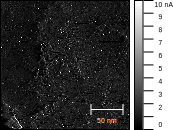
\includegraphics[width=.5\textwidth]{../data/Gold_200nm_current.png}
        \caption{Gold: Stromkarte im const. current Modus (Setpoint=\SI{1}{\nano A}, P-Gain=\SI{1000}{}, I-Gain=\SI{2000}{} und Tip voltage=\SI{1}{V})} \label{fig:g200nmc}
\end{figure}
\begin{figure}[h]
        \centering
        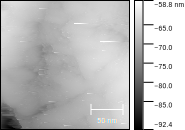
\includegraphics[width=.5\textwidth]{../data/Gold_200nm_z.png}
        \caption{Gold: Höhenkarte im const. current Modus (Setpoint=\SI{1}{\nano A}, P-Gain=\SI{1000}{}, I-Gain=\SI{2000}{} und Tip voltage=\SI{1}{V})} \label{fig:g200nmz}
\end{figure}
\begin{figure}[h]
        \centering
        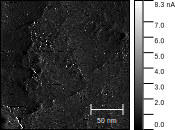
\includegraphics[width=.5\textwidth]{../data/Gold_200nm_50mV_current.png}
        \caption{Gold: Stromkarte im const. current Modus (Setpoint=\SI{1}{\nano A}, P-Gain=\SI{1000}{}, I-Gain=\SI{2000}{} und Tip voltage=\SI{50}{\milli V})} \label{fig:g200nm50mVc}
\end{figure}
\begin{figure}[h]
        \centering
        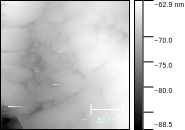
\includegraphics[width=.5\textwidth]{../data/Gold_200nm_50mV_z.png}
        \caption{Gold: Höhenkarte im const. current Modus (Setpoint=\SI{1}{\nano A}, P-Gain=\SI{1000}{}, I-Gain=\SI{2000}{} und Tip voltage=\SI{50}{\milli V})} \label{fig:g200nm50mVz}
\end{figure}
\begin{figure}[h]
        \centering
        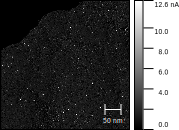
\includegraphics[width=.5\textwidth]{../data/Gold_400nm_current.png}
        \caption{Gold: Stromkarte im const. current Modus (Setpoint=\SI{1}{\nano A}, P-Gain=\SI{1000}{}, I-Gain=\SI{2000}{} und Tip voltage=\SI{1}{V})} \label{fig:g400nmc}
\end{figure}
\begin{figure}[h]
        \centering
        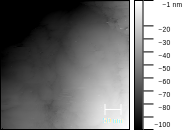
\includegraphics[width=.5\textwidth]{../data/Gold_400nm_z.png}
        \caption{Gold: Höhenkarte im const. current Modus (Setpoint=\SI{1}{\nano A}, P-Gain=\SI{1000}{}, I-Gain=\SI{2000}{} und Tip voltage=\SI{1}{V})} \label{fig:g400nmz}
\end{figure}

\clearpage
\section{HOPG}
% TODO: Beachte, dass die beiden pngs hier mit 1V benannte sind, aber eigentlich 50mV Tip voltage hatten
\begin{figure}[h]
        \centering
        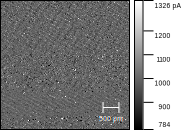
\includegraphics[width=.5\textwidth]{../data/Graphit_4nm_1V_current.png}
        \caption{HOPG: Stromkarte im const. current Modus (Setpoint=\SI{1}{\nano A}, P-Gain=\SI{1000}{}, I-Gain=\SI{2000}{} und Tip voltage=\SI{50}{\nano V})} \label{fig:gr4nm50nVc}
\end{figure}
\begin{figure}[h]
        \centering
        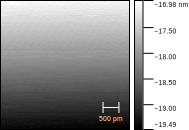
\includegraphics[width=.5\textwidth]{../data/Graphit_4nm_1V_z.png}
        \caption{HOPG: Höhenkarte im const. current Modus (Setpoint=\SI{1}{\nano A}, P-Gain=\SI{1000}{}, I-Gain=\SI{2000}{} und Tip voltage=\SI{50}{\nano V})} \label{fig:gr4nm50nVz}
\end{figure}
\begin{figure}[h]
        \centering
        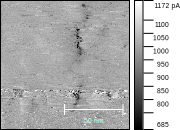
\includegraphics[width=.5\textwidth]{../data/Graphit2_current.png}
        \caption{HOPG: Stromkarte im const. current Modus (Setpoint=\SI{1}{\nano A}, P-Gain=\SI{1000}{}, I-Gain=\SI{2000}{} und Tip voltage=\SI{100}{\nano V})} \label{fig:gr100nm100nVc}
\end{figure}
\begin{figure}[h]
        \centering
        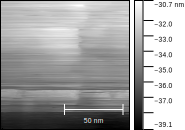
\includegraphics[width=.5\textwidth]{../data/Graphit2_z.png}
        \caption{HOPG: Höhenkarte im const. current Modus (Setpoint=\SI{1}{\nano A}, P-Gain=\SI{1000}{}, I-Gain=\SI{2000}{} und Tip voltage=\SI{100}{\nano V})} \label{fig:gr100nm100nVz}
\end{figure}
\begin{figure}[h]
        \centering
        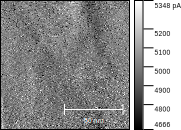
\includegraphics[width=.5\textwidth]{../data/Graphit3_current.png}
        \caption{HOPG: Stromkarte im const. current Modus (Setpoint=\SI{5}{\nano A}, P-Gain=\SI{1000}{}, I-Gain=\SI{2000}{} und Tip voltage=\SI{200}{\nano V})} \label{fig:gr100nm200nVc}
\end{figure}
\begin{figure}[h]
        \centering
        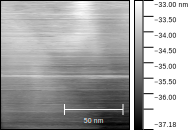
\includegraphics[width=.5\textwidth]{../data/Graphit3_z.png}
        \caption{HOPG: Höhenkarte im const. current Modus (Setpoint=\SI{5}{\nano A}, P-Gain=\SI{1000}{}, I-Gain=\SI{2000}{} und Tip voltage=\SI{200}{\nano V})} \label{fig:gr100nm200nVz}
\end{figure}
\begin{figure}[h]
        \centering
        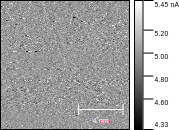
\includegraphics[width=.5\textwidth]{../data/Graphit4_current.png}
        \caption{HOPG: Stromkarte im const. current Modus (Setpoint=\SI{5}{\nano A}, P-Gain=\SI{1000}{}, I-Gain=\SI{2000}{} und Tip voltage=\SI{200}{\nano V})} \label{fig:gr10nm200nVc}
\end{figure}
\begin{figure}[h]
        \centering
        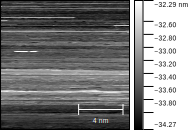
\includegraphics[width=.5\textwidth]{../data/Graphit4_z.png}
        \caption{HOPG: Höhenkarte im const. current Modus (Setpoint=\SI{5}{\nano A}, P-Gain=\SI{1000}{}, I-Gain=\SI{2000}{} und Tip voltage=\SI{200}{\nano V})} \label{fig:gr10nm200nVz}
\end{figure}
\begin{figure}[h]
        \centering
        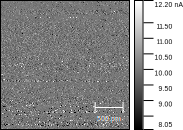
\includegraphics[width=.5\textwidth]{../data/Graphit5_current.png}
        \caption{HOPG: Stromkarte im const. current Modus (Setpoint=\SI{1}{\nano A}, P-Gain=\SI{1000}{}, I-Gain=\SI{2000}{} und Tip voltage=\SI{50}{\nano V})} \label{fig:gr2nm50nVc}
\end{figure}
\begin{figure}[h]
        \centering
        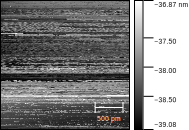
\includegraphics[width=.5\textwidth]{../data/Graphit5_z.png}
        \caption{HOPG: Höhenkarte im const. current Modus (Setpoint=\SI{1}{\nano A}, P-Gain=\SI{1000}{}, I-Gain=\SI{2000}{} und Tip voltage=\SI{50}{\nano V})} \label{fig:gr2nm50nVz}
\end{figure}
\begin{figure}[h]
        \centering
        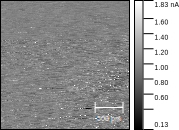
\includegraphics[width=.5\textwidth]{../data/Graphit6_current.png}
        \caption{HOPG: Stromkarte im const. current Modus (Setpoint=\SI{1}{\nano A}, P-Gain=\SI{1000}{}, I-Gain=\SI{2000}{} und Tip voltage=\SI{50}{\nano V})} \label{fig:gr2nm50nVc2}
\end{figure}
\begin{figure}[h]
        \centering
        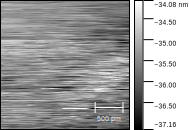
\includegraphics[width=.5\textwidth]{../data/Graphit6_z.png}
        \caption{HOPG: Höhenkarte im const. current Modus (Setpoint=\SI{1}{\nano A}, P-Gain=\SI{1000}{}, I-Gain=\SI{2000}{} und Tip voltage=\SI{50}{\nano V})} \label{fig:gr2nm50nVz2}
\end{figure}
\begin{figure}[h]
        \centering
        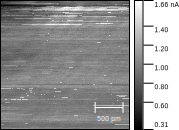
\includegraphics[width=.5\textwidth]{../data/Graphit7_current.png}
        \caption{HOPG: Stromkarte im const. current Modus (Setpoint=\SI{1}{\nano A}, P-Gain=\SI{1000}{}, I-Gain=\SI{2000}{} und Tip voltage=\SI{50}{\nano V})} \label{fig:gr2nm50nVc3}
\end{figure}
\begin{figure}[h]
        \centering
        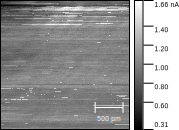
\includegraphics[width=.5\textwidth]{../data/Graphit7_z.png}
        \caption{HOPG: Höhenkarte im const. current Modus (Setpoint=\SI{1}{\nano A}, P-Gain=\SI{0}{}, I-Gain=\SI{4}{} und Tip voltage=\SI{50}{\nano V})} \label{fig:gr2nm50nVz3}
\end{figure}
\begin{figure}[h]
  \centering
  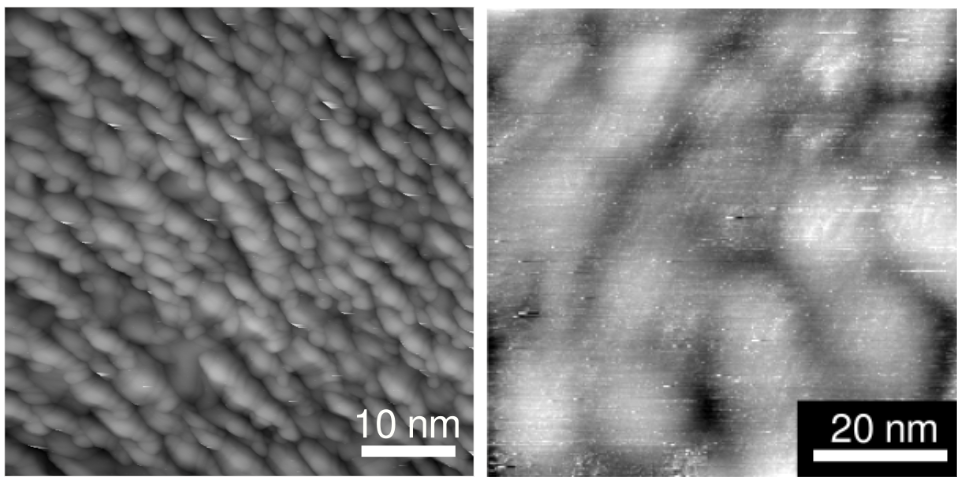
\includegraphics[width=.5\textwidth]{422_gold_lit.png}
  \caption{Literaturbild der Goldprobe aus \cite{anleitung422}.} \label{fig:gold_lit}
\end{figure}
\begin{figure}[h]
  \centering
  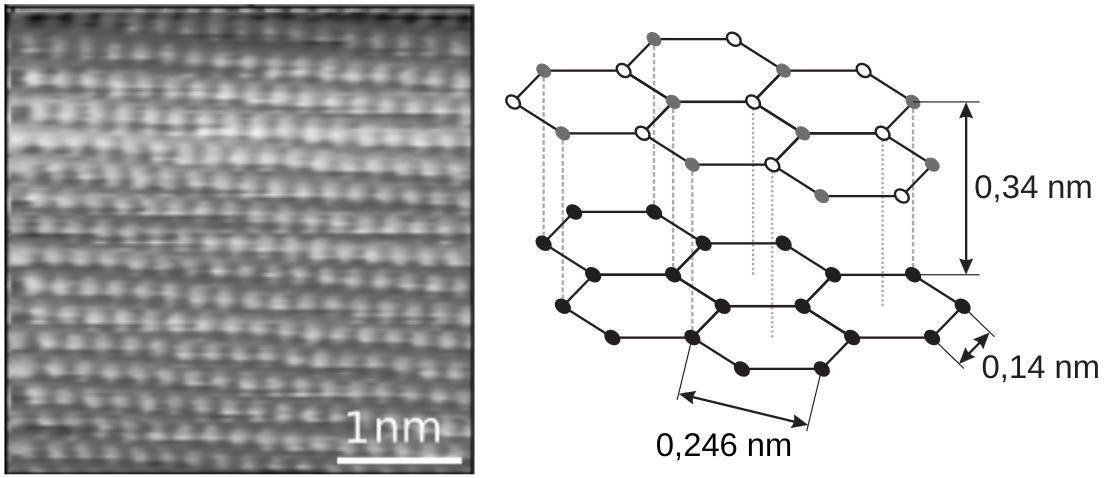
\includegraphics[width=.5\textwidth]{422_HOPG_lit.png}
  \caption{Literaturbild der HOPG Probe aus \cite{anleitung422}.} \label{fig:hopg_lit}
\end{figure}
\begin{figure}[h]
  \centering
  \includegraphics[width=.5\textwidth]{../data/gold_1_norm.png}
  \caption{Gitter zur Bestimmung des Maßstabs (fern).} \label{fig:gitter_fern}
\end{figure}
\begin{figure}[h]
  \centering
  \includegraphics[width=.5\textwidth]{../data/gold_3_norm.png}
  \caption{Gitter zur Bestimmung des Maßstabs (nah).} \label{fig:gitter_nah}
\end{figure}


\end{document}
